\section{Неориентированные графы}
\label{sec:graphs}

\defemph{Графы}~--- это математические объекты, довольно часто встречающиеся в реальных задачах (логистика, интернет, социальные связи),
но при этом достаточно простые, чтобы без труда формально определить их при помощи изученного нами математического аппарата.
Неформально говоря, граф~--- это абстракция, применимая к множеству любой природы, в случае, когда интересны только парные связи между его элементами.

Граф часто представляется в виде изображения следующего формата: точки или кружки (элементы множества, \defemph{вершины}) соединены линиями или стрелками (\defemph{рёбрами}),
изображающими связи между элементами.
Вершины и рёбра могут иметь некоторые \defemph{атрибуты} (числа, строки, любые другие объекты).

\begin{figure}[ht!]
    \center
    \begin{tikzpicture}
        \node[shape=circle,draw=black] (NK)  at (1,0) {НК};
        \node[shape=circle,draw=black] (KPM) at (-1,-1) {КПМ};
        \node[shape=circle,draw=black] (GK)  at (3,2) {ГК};
        \node[shape=circle,draw=black] (DIG) at (2,4) {Цифра};
        \node[shape=circle,draw=black] (ARK) at (0,6) {Арктика};
        \node[shape=circle,draw=black] (LK)  at (5,2) {ЛК};
        \node[shape=circle,draw=black] (AC)  at (7,0) {АК};
        \node[shape=circle,draw=black] (KSP) at (6,-2) {КСП};
        \node[shape=rectangle,draw=black] (ARMY) at (11,0) {Военкомат};

        \path [-] (NK) edge node[sloped, anchor=center, above] {$500$}  (KPM);
        \path [-] (NK) edge node[sloped, anchor=center, above] {$1500$} (GK);
        \path [-] (GK) edge node[sloped, anchor=center, above] {$700$}  (DIG);
        \path [-] (GK) edge node[sloped, anchor=center, above] {$400$}  (LK);
        \path [-] (DIG)edge node[sloped, anchor=center, above] {$300$}  (ARK);
        \path [-, dashed](LK) edge node[sloped, anchor=center, above] {$500$} (AC);
        \path [<->, dashed](AC) edge node[sloped, anchor=center, above] {$450$} (KSP);
        \path [<->, dashed](NK) edge [bend left=-30] node[sloped, anchor=center, above] {$600$} (KSP);
        \path [->, dashed](AC) edge node[sloped, anchor=center, above] {$0.1$} (ARMY);
    \end{tikzpicture}

    \label{fig:graphs:people_phystech}
    \caption{граф ежедневного перемещения людей между некоторыми связанными с Физтехом зданиями.
    Рёбра обозначают тип и направление перехода, а также ежедневный поток студентов.}
\end{figure}


Изучение графов мы начнём с самых простых их разновидностей, постепенно усложняя конструкцию.
Но перед этим потребуется ввести пару вспомогательных определений.

\begin{definition}
    \defemph{Множеством всех подмножеств мощности $ k $} некоторого множества $ A $ будем называть множество
    \[
        \binom{A}{k}
        =
        \{ B \mid (B \subseteq A) \wedge (|B| = k) \}
    \]
\end{definition}

\begin{definition}
    \defemph{Множеством всех неупорядоченных пар} некоторого множества $ A $ будем называть множество $ \displaystyle \begin{pmatrix} A \\ 2 \end{pmatrix} $.
\end{definition}

\begin{remark}
    \label{remark:graphs:subsets_cardinality}
    Если $ |A| = n < +\infty $, и $ 0 \leqslant k \leqslant n $, то
    \[
        \left|
        \binom{A}{k}
        \right|
        =
        \frac{n!}{k! (n-k)!}
        \defeq
        \binom{n}{k}
        \defeq
        C_n^k
    \]
\end{remark}



\subsection{Простые неориентированные графы}
\label{subsec:graphs:simple_graphs}

%Начнём с \defemph{простых неориентированных графов}, то есть, с графов, вершины и рёбра которых не имеют никаких атрибутов (в том числе, направления).
Начнём с самой простой конструкции графа, для построения которой достаточно понятия неупорядоченной пары.
\begin{definition}
    \defemph{(Простой неориентированный) граф}~--- это упорядоченная пара $ (V, E) $ множества \defemph{вершин} $ V $
    и \defemph{рёбер} $ E \subseteq \binom{V}{2} $.
    Введём также следующие обозначения, если $ V $ и $ E $ фиксированы:
    \[
        G = (V, E)\text{~--- граф} \qquad \Longrightarrow \qquad
        G(V, E) \defeq (V, E), \; V(G) \defeq V, \; E(G) \defeq E
    \]
\end{definition}

\defemph{<<Простой>>} означает, что в графе нет \defemph{петель} (рёбер вида $ \{v, \; v\} = \{ v \} $) и \defemph{кратных рёбер} (каждое ребро входит в $ E $ единожды).
\defemph{<<Неориентированный>>} означает, что ребро является неупорядоченной парой.


Зафиксируем граф $ G = G(V, E) $.
\begin{definition}
    Вершины $ u $ и $ v $ называются \defemph{смежными} или \defemph{соседями}, если они образуют ребро: $ \{u, v\} \in E $.
    Рёбра $ e $ и $ f $ называются \defemph{смежными}, если они имеют общую вершину: $ e \cap f \neq \varnothing $.
    Вершина $ v $ \defemph{инцидента} ребру $ e $, если $ u \in e $.
    Вершины $ u $ и $ v $, инцидентные ребру $ e $, называются его \defemph{концами};
    говорят, что $ e $ \defemph{соединяет} $ u $ и $ v $.
    \newline
    Рёбра часто записывают сокращённо: $ uv $ вместо $ \{u, v\} $.
\end{definition}

\begin{definition}
    \defemph{Степенью} вершины $ v $ называется число $ d(v) $ смежных с $ v $ рёбер.
\end{definition}

\begin{theorem}[о рукопожатиях]
    \label{theorem:graphs:sum_of_degs}
    $ \displaystyle \sum_{v \in V} d(V) = 2 |E| $
\end{theorem}

\begin{proof}
    $ \displaystyle \sum_{v \in V} d(V) = \sum_{v \in V} \sum_{\substack{e \in E, \\ v \in e}} 1 = \sum_{e \in E} \sum_{\substack{v \in V, \\ v \in e}} 1 = \sum_{e \in E} 2 = 2 |E| $
\end{proof}

Определим отдельно несколько частных случаев простого неориентированного графа.
\begin{definition}
    \begin{enumerate}[label=\arabic*)]
        \item[]
        \item
            \defemph{Граф-путь} $ P_n $, $ n \geqslant 0 $~--- граф вида
            \[
                V(P_n) = \{ v_1, \ldots, v_n \}, \qquad
                E(P_n) = \left\{ \{v_0, v_1\}, \{v_1, v_2\}, \ldots, \{v_{n-1}, v_n\} \right\}
            \]
            Вершины $ v_1 $ и $ v_n $ называются \defemph{концами пути}, а $ n = |E| $~--- \defemph{длиной}.
            \textit{Ещё раз акцентируем внимание на том, что $ n \geqslant 0 $, а вершины нумеруются с нуля.}
        \item
            \defemph{Граф-цикл} $ C_n $, $ n \geqslant 3 $~--- граф вида
            \[
                V(G) = \{ v_1, \ldots, v_n \}, \qquad
                E(G) = \left\{ \{v_1, v_2\}, \{v_2, v_3\}, \ldots, \{v_{n-1}, v_n\}, \{v_n, v_1\} \right\}
            \]
            \textit{Ещё раз акцентируем внимание на том, что $ n \geqslant 3 $.}
        \item
            \defemph{Полный граф} (или \defemph{граф-клика}) $ K_n(V, E) $, $ n \geqslant 1 $~--- это граф, заданный равенством
            \[
                K_n(V, E) = \left( V, \binom{V}{2} \right), \; n = |V| \qquad \left(\text{ то есть } E = \binom{V}{2} \right)
            \]
        \item
            \defemph{Граф-звезда} $ S_n $, $ n \geqslant 0 $~--- граф вида
            \[
                V(S_n) = \{ v_0, v_1, \ldots, v_n \} \qquad
                E(S_n) = \left\{ \{v_0, v_1\}, \{v_0, v_2\}, \ldots, \{v_0, v_n\} \right\}
            \]
            \textit{Ещё раз акцентируем внимание на том, что $ n \geqslant 0 $, а вершины нумеруются с нуля.}
        \item
            \defemph{Пустой граф}~--- граф, у которого $ V = E = \varnothing $.
            Его принято обозначать тоже $ \varnothing $, хотя, формально, это $ (\varnothing, \varnothing) \neq \varnothing $.
    \end{enumerate}
\end{definition}

\begin{figure}[ht!]
    \center
    \raisebox{-0.5\height}{  % Центрирование по вертикали.
    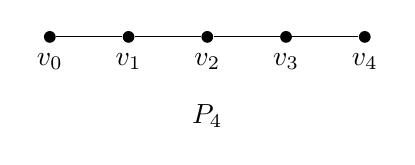
\begin{tikzpicture}
        \node[circle,fill,inner sep=1.5pt,label=below:$v_0$] (v0)  at (0,0) {};
        \node[circle,fill,inner sep=1.5pt,label=below:$v_1$] (v1)  at (1,0) {};
        \node[circle,fill,inner sep=1.5pt,label=below:$v_2$] (v2)  at (2,0) {};
        \node[circle,fill,inner sep=1.5pt,label=below:$v_3$] (v3)  at (3,0) {};
        \node[circle,fill,inner sep=1.5pt,label=below:$v_4$] (v4)  at (4,0) {};
        \node (P4) at (2,-1) {$ P_4 $};

        \path [-] (v0) edge node {}  (v1);
        \path [-] (v1) edge node {}  (v2);
        \path [-] (v2) edge node {}  (v3);
        \path [-] (v3) edge node {}  (v4);
    \end{tikzpicture}
    }%
    %
    \hspace{2\baselineskip}%
    %
    \raisebox{-0.5\height}{
    \begin{tikzpicture}
        \node[circle,fill,inner sep=1.5pt,label=below:$v_1$] (v1)  at (-54:2) {};
        \node[circle,fill,inner sep=1.5pt,label=right:$v_2$] (v2)  at (18:2)  {};
        \node[circle,fill,inner sep=1.5pt,label=above:$v_3$] (v3)  at (90:2)  {};
        \node[circle,fill,inner sep=1.5pt,label=left:$v_4$]  (v4)  at (162:2) {};
        \node[circle,fill,inner sep=1.5pt,label=below:$v_5$] (v5)  at (234:2) {};
        \node (C5) at (0,-2.5) {$ C_5 $};

        \path [-] (v1) edge node {}  (v2);
        \path [-] (v2) edge node {}  (v3);
        \path [-] (v3) edge node {}  (v4);
        \path [-] (v4) edge node {}  (v5);
        \path [-] (v5) edge node {}  (v1);
    \end{tikzpicture}
    }%

    \vspace{\baselineskip}

    \raisebox{-0.5\height}{
    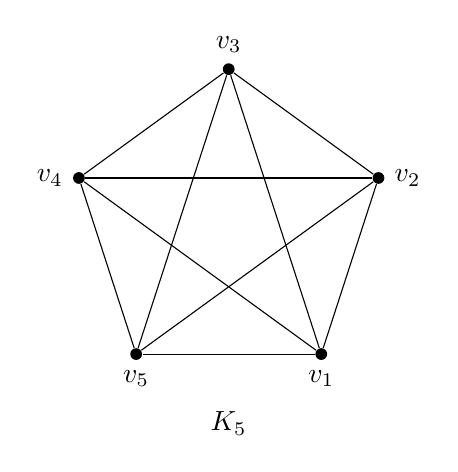
\begin{tikzpicture}
        \node[circle,fill,inner sep=1.5pt,label=below:$v_1$] (v1)  at (-54:2) {};
        \node[circle,fill,inner sep=1.5pt,label=right:$v_2$] (v2)  at (18:2)  {};
        \node[circle,fill,inner sep=1.5pt,label=above:$v_3$] (v3)  at (90:2)  {};
        \node[circle,fill,inner sep=1.5pt,label=left:$v_4$]  (v4)  at (162:2) {};
        \node[circle,fill,inner sep=1.5pt,label=below:$v_5$] (v5)  at (234:2) {};
        \node (K5) at (0,-2.5) {$ K_5 $};

        \path [-] (v1) edge node {}  (v2);
        \path [-] (v1) edge node {}  (v3);
        \path [-] (v1) edge node {}  (v4);
        \path [-] (v1) edge node {}  (v5);
        \path [-] (v2) edge node {}  (v3);
        \path [-] (v2) edge node {}  (v4);
        \path [-] (v2) edge node {}  (v5);
        \path [-] (v3) edge node {}  (v4);
        \path [-] (v3) edge node {}  (v5);
        \path [-] (v4) edge node {}  (v5);
    \end{tikzpicture}
    }%
    %
    \hspace{2\baselineskip}%
    %
    \raisebox{-0.5\height}{
    \begin{tikzpicture}
        \node[circle,fill,inner sep=1.5pt,label={[label distance = 5]below:$v_0$}] (v0)  at (0,0) {};
        \node[circle,fill,inner sep=1.5pt,label=below:$v_1$] (v1)  at (-54:2) {};
        \node[circle,fill,inner sep=1.5pt,label=right:$v_2$] (v2)  at (18:2)  {};
        \node[circle,fill,inner sep=1.5pt,label=above:$v_3$] (v3)  at (90:2)  {};
        \node[circle,fill,inner sep=1.5pt,label=left:$v_4$]  (v4)  at (162:2) {};
        \node[circle,fill,inner sep=1.5pt,label=below:$v_5$] (v5)  at (234:2) {};
        \node (S5) at (0,-2.5) {$ S_5 $};

        \path [-] (v0) edge node {}  (v1);
        \path [-] (v0) edge node {}  (v2);
        \path [-] (v0) edge node {}  (v3);
        \path [-] (v0) edge node {}  (v4);
        \path [-] (v0) edge node {}  (v5);
    \end{tikzpicture}
    }%

    \label{fig:graphs:basic_graphs}
    \caption{базовые графы}
\end{figure}



\subsection{Теоретико-множественные операции с графами}
\label{subsec:graphs:graph_operations}

Известные нам теоретико-множественные операции можно обобщить на графы.
\begin{definition}
    Пусть $ G(V, E) $ и $ H(W, I) $~--- графы.
    Тогда \defemph{объединение}, \defemph{персечение} $ G $ и $ H $, а также \defemph{дополнение} $ G $ определяются как, соответственно,
    \[
        G \cup H = \left( V \cup W, E \cup I \right), \quad
        G \cap H = \left( V \cap W, E \cap I \right), \quad
        G^c = \left( V, \binom{V}{2} \setminus E \right)
    \]
    Множество $ \binom{V}{2} \setminus E $ называется множеством \defemph{нерёбер} графа $ G(V, E) $.
\end{definition}

\begin{remark}
    \label{remark:graphs:complement}
    $ G \cup G^c = K_{|V(G)|} $.
\end{remark}

\begin{Exercise}[counter=SecExercise]
    \noindent
    Существует ли такой граф-цикл, дополнение которого тоже является графом-циклом?
\end{Exercise}

\begin{Answer}
    \noindent
    Так как при дополнении число вершин не меняется, если такой граф и есть, то, в силу \ref{remark:graphs:subsets_cardinality} и \ref{remark:graphs:complement}, выполено равенство
    \[
        |V(C_n)| = n = \frac{n(n-1)}{2} - n = |V(K_n)| - |V(C_n)|, \qquad n \geqslant 1
    \]
    Отсюда $ n = 5 $.
    Тогда легко привести единственный пример такого графа:
    \begin{center}
    \raisebox{-0.5\height}{
    \begin{tikzpicture}
        \node[circle,fill,inner sep=1.5pt,label=below:$v_1$] (v1)  at (-54:2) {};
        \node[circle,fill,inner sep=1.5pt,label=right:$v_2$] (v2)  at (18:2)  {};
        \node[circle,fill,inner sep=1.5pt,label=above:$v_3$] (v3)  at (90:2)  {};
        \node[circle,fill,inner sep=1.5pt,label=left:$v_4$]  (v4)  at (162:2) {};
        \node[circle,fill,inner sep=1.5pt,label=below:$v_5$] (v5)  at (234:2) {};
        \node (C5) at (0,-2.5) {$ C_5 $};

        \path [-] (v1) edge node {}  (v2);
        \path [-] (v2) edge node {}  (v3);
        \path [-] (v3) edge node {}  (v4);
        \path [-] (v4) edge node {}  (v5);
        \path [-] (v5) edge node {}  (v1);
    \end{tikzpicture}
    }%
    %
    \hspace{2\baselineskip}
    %
    \raisebox{-0.5\height}{
    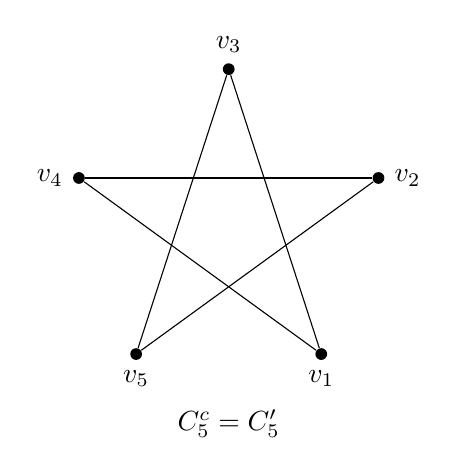
\begin{tikzpicture}
        \node[circle,fill,inner sep=1.5pt,label=below:$v_1$] (v1)  at (-54:2) {};
        \node[circle,fill,inner sep=1.5pt,label=right:$v_2$] (v2)  at (18:2)  {};
        \node[circle,fill,inner sep=1.5pt,label=above:$v_3$] (v3)  at (90:2)  {};
        \node[circle,fill,inner sep=1.5pt,label=left:$v_4$]  (v4)  at (162:2) {};
        \node[circle,fill,inner sep=1.5pt,label=below:$v_5$] (v5)  at (234:2) {};
        \node (C5c) at (0,-2.5) {$ C_5^c = C'_5 $};

        \path [-] (v1) edge node {}  (v3);
        \path [-] (v1) edge node {}  (v4);
        \path [-] (v2) edge node {}  (v4);
        \path [-] (v2) edge node {}  (v5);
        \path [-] (v3) edge node {}  (v5);
    \end{tikzpicture}
    }%

    \end{center}
\end{Answer}



\subsection{Подграфы}
\label{subsec:graphs:subgraphs}

Иногда бывает интересно исследовать какую-то часть графа как отдельный граф.
Это может понадобиться как при решении реальных задач, так и при доказательстве вспомогательных фактов.

\begin{definition}
    Граф $ H(W, I) $ является \defemph{(рёберным) подграфом} графа $ G(V, E) $ $ \defarr $ $ W \subseteq V $ и $ I \subseteq E $.
    Это обозначается как $ H \subseteq G $.
    Случай, когда $ H \subseteq G $ и $ H \neq G $, обозначается как $ H \varsubsetneq G $.
    Если при этом ещё и $ H \neq \varnothing $, $ H \neq G $, то подграф называется \defemph{несобственным}.
\end{definition}

\begin{definition}
    Пусть $ G(V, E) $~--- граф, $ U \subseteq V $.
    Будем называть \defemph{индуцированным (множеством $ U $) подграфом} граф $ \left( U, \binom{U}{2} \cap E \right) $.
    Индуцированный подграф обозначается $ H[U] $.
\end{definition}

Неформально, индуцированный множеством $ U $ подграф~--- это подграф на вершинах $ U $, в ктором провели все возможные рёбра, которые есть в исходном графе.

\begin{definition}
    Множество $ U \subseteq V $ называется \defemph{независимым} множеством вершин графа $ G(V, E) $ $ \defarr $ $ H[U] $ не содержит рёбер.
\end{definition}

\begin{definition}
    \defemph{Подграфом-путём}/\defemph{циклом}/\defemph{кликой}/\defemph{звездой} некоторого графа $ G $ называется подграф $ G $,
    являющийся путём/циклом/полным графом/звездой соответственно.
\end{definition}

Данное определение естественным образом обобщается и на любые другие именные частные случаи графов.

\begin{definition}
    Пусть предикат $ P(x) $ определён на множестве графов (он задаёт некоторое свойство/определение, см. \ref{definition:formal_systems:definition}).
    Обозначим $ P_G = \{ x \subseteq G \mid P(x) \} $ множество всех подграфов графа $ G $, удовлетворяющих свойству $ P(x) $.
    \newline
    Подграф $ H \in P_G $ является \defemph{максимальным} среди подграфов со свойством $ P $ $ \defarr $ $ \forall H' \in P_G \;\; (H \subseteq H') \rightarrow (H = H') $.
\end{definition}

\begin{Exercise}[counter=SecExercise, label=exercise:graphs:is_maximal]
    \noindent
    Верно ли, что определение максимального подграфа со свойством $ P $ эквивалентно следующему:
    $ H \in P_G $~--- максимальный подграф графа $ G $ со свойством $ P $ $ \defarr $ $ \forall H' \in P_G \;\; H' \subseteq H $?
\end{Exercise}

\begin{Answer}
    \noindent
    Нет, неверно.
    В частности, если рассмотреть $ G = P_2 \sqcup P'_1 $%
    \footnote{Операция $ \sqcup $ означает то же самое, что и $ \cup $, просто с такой записью уточняется, что объединяемые множества не пересекаются.},
    то максимальным подграфом-путём в нём будет $ P_2 $, но определению из условия задачи он удовлетворять не будет,
    так как $ P'_1 \not\subseteq P_2 $.
\end{Answer}



\subsection{Связность}
\label{subsec:graphs:connectivity}

Граф, полученный в решении задачи \ref{exercise:graphs:is_maximal}, состоит как бы из двух <<независимых>>, или \defemph{несвязных} подграфов $ P_2 $ и $ P'_1 $.
В реальных задачах часто требуется обнаружить подобные случаи (например, чтобы определить недостижимые части страны по карте дорог, или отдельные социальные группы по графу связей).

\begin{definition}
    Вершина $ u $ в графе $ G $ является \defemph{достижимой} из вершины $ v $ $ \defarr $ существует подграф-путь графа $ G $, концами которого являются вершины $ u $ и $ v $.
    Это обозначается как $ u \leadsto v $.
\end{definition}

\begin{remark}
    \label{remark:graphs:connectivity_relation}
    В случае неориентированного графа $ (u \leadsto v) \leftrightarrow (v \leadsto u) $ (\defemph{симметричность} достижимости).
    \newline
    Также $ u \leadsto u $ (\defemph{рефлексивность}) и $ \left[ (u \leadsto v) \wedge (v \leadsto w) \right] \rightarrow (u \leadsto w) $ (\defemph{транзитивность}).
\end{remark}

\begin{definition}
    \label{definition:graphs:connectivity_component}
    \defemph{Компонентой связности} графа $ G(V, E) $ будем называть подграф $ G $, индуцированный на некотором \underline{непустом} множестве $ U \subseteq V $,
    удовлетворяющем свойству $ \forall u, v \in U \; (u \leadsto v) $ и являющемся максимальным относительно него.
    \newline
    Компонента связности, состоящая из одной вершины, называется \defemph{изолированной вершиной}.
    \newline
    Граф, являющийся компонентой связности самого себя, называется \defemph{связным}.
\end{definition}

\begin{remark}
    \label{remark:graphs:cc_partition}
    Позже будет доказано, что из замечания \ref{remark:graphs:connectivity_relation} следует, что любой граф разбивается на компоненты связности, причём единственным образом:
    \[
        G = H_1 \sqcup H_2 \sqcup \ldots \sqcup H_k
    \]
\end{remark}

\begin{Exercise}[counter=SecExercise]
    \noindent
    Пусть $ G $ и $ H $~--- простые графы, причём $ G \cap H = \varnothing $.
    Определим граф $ G \times H $ следующим образом:
    \[
        V(G \times H) = \left\{ \{u, v\} \mid u \in V(G), v \in V(H) \right\}
    \]
    \begin{multline*}
        %E(G \times H) = \Big\{ \big\{ \{u_1, v_1 \}, \{u_2, v_2 \} \big\} \, \Big| \, \left( \{u_1, u_2\} \in E(G) \right) \wedge \left( \{v_1, v_2\} \in E(H) \right) \Big\}
        E(G \times H) = \Big\{ \big\{ \{u_1, v \}, \{u_2, v \} \big\} \, \Big| \, \left( \{u_1, u_2\} \in E(G) \right) \wedge \left( v \in V(H) \right) \Big\} \cup \\
        \cup \Big\{ \big\{ \{u, v_1 \}, \{u, v_2 \} \big\} \, \Big| \, \left( \{v_1, v_2\} \in E(H) \right) \wedge \left( u \in V(G) \right) \Big\}
    \end{multline*}
    Пусть $ G $ имеет $ n $ компонент связности, а $ H $~--- $ m $.
    Сколько компонент связности имеет $ G \times H $?
    Как они устроены?
\end{Exercise}

\begin{Answer}
    \noindent
    Заметим, что $ \{ u_1, v_1 \} \leadsto \{ u_2, v_2 \} \; \Longleftrightarrow \; (u_1 \leadsto u_2) \wedge (v_1 \leadsto v_2) $.
    \newline
    Действительно,
    \begin{enumerate}
        \item[$ \Leftarrow $]
            Если $ u_1 \leadsto u_k $ и $ v_1 \leadsto v_l $, то существуют пути $ P_G $ и $ P_H $ из $ u_1 $ в $ u_k $ и из $ v_1 $ в $ v_l $ соответственно
            (нумерация введена уже для вершин путей).

            Заметим, что все рёбра вида $ \big \{ \{u_i, v_j\}, \{u_{i+1}, v_j\} \big \} $ и $ \big \{ \{u_i, v_j\}, \{u_i, v_{j+1}\} \big \} $,
            где $ \{ u_i, u_{i+1} \} \in E(P_G) $ и $ \{ v_j, v_{j+1} \} \in E(P_H) $,
            лежат в $ E(G \times H) $ по построению.

            Но тогда в $ G \times H $ есть путь вида
            \[
                \{ u_1, v_1 \} \to \{ u_2, v_1 \} \to \ldots \to \{ u_k, v_1 \} \to \{ u_k, v_2 \} \to \ldots \to \{ u_k, v_l \}
            \]
            То есть $ \{ u_1, v_1 \} \leadsto \{ u_k, v_l \} $.
        \item[$ \Rightarrow $]
            Если $ \{ u_1, v_1 \} \leadsto \{ u_k, v_l \} $, то существует путь $ P_{G \times H} $ из $  \{ u_1, v_1 \} $ в $ \{ u_k, v_l \} $.

            Из определения $ G \times H $ следует, можно перенумеровать $ u_i $ и $ u_j $ так, что путь $ P_{G \times H} $ имеет рёбра только вида
            $ \big \{ \{u_i, v_j\}, \{u_{i+1}, v_j\} \big \} $ или $ \big \{ \{u_i, v_j\}, \{u_i, v_{j+1}\} \big \} $.

            Но тогда в $ G $ и $ H $ есть пути $ u_1 \to u_2 \to \ldots \to u_k $ и $ v_1 \to v_2 \to \ldots \to v_l $ соответственно.
            То есть $ u_1 \leadsto u_k $ и $ v_1 \leadsto v_l $.
    \end{enumerate}
    Но тогда получаем, что все компоненты связности графа $ G \times H $ будут иметь вид $ G_i \times H_j $,
    где $ G_i $ и $ H_j $~--- компоненты связности графов $ G $ и $ H $ соответственно.
    Тогда ответ: $ n \cdot m $.
\end{Answer}



\subsection{Деревья}
\label{subsec:graphs:trees}

Часто бывает удобно исследовать, в некотором смысле, \defemph{минимальные} по числу рёбер связные графы.
Такие графы называются \defemph{деревьями} и обладают множеством полезных свойств.

\begin{definition}
    \defemph{Деревом} назовём \defemph{минимально связный граф}, то есть граф, теряющий свойство связности при удалении любого ребра.
\end{definition}

Если подходить к деревьям именно со стороны минимальности, то кажется осмысленным сначала привести некоторую оценку,
насколько вообще можно сделать <<малым>> граф, сохраняя его связность.

\begin{theorem}
    Пусть $ \text{\#КС}(G) $ обозначает число компонент связности некоторого графа $ G(V, E) $.
    Тогда $ \forall G \;\, \text{\#КС}(G) \geqslant |V(G)| - |E(G)| $.
\end{theorem}

\begin{proof}
    По индукции для фиксированного $ |V| $ по числу рёбер от $ 0 $ до $ |V| $.
\end{proof}

\begin{corollary}
    Если граф связный, то $ |E| \geqslant |V| - 1 $.
\end{corollary}

Из следствия очевидным образом можно получить эквивалентное определение дерева.
На самом деле, этим множество эквивалентных определения дерева не ограничивается.

\begin{theorem}
    \label{theorem:graphs:trees_defs}
    Следующие свойства эквивалентны:
    \begin{enumerate}[label=(\arabic*)]
        \item
            Граф $ G(V,E) $ минимально связный.
        \item
            \label{item:graphs:e_v_minus_one}
            Граф $ G(V,E) $ связный и $ |E| = |V| - 1 $.
        \item
            Граф $ G(V,E) $ связный и \defemph{ациклический} (не имеет подграфов-циклов).
        \item
            В графе $ G(V,E) $ из любой вершины в любую есть путь, причём единственный.
    \end{enumerate}
\end{theorem}

В ходе доказательства теоремы выше обычно используется следующая (полезная и в отдельности) лемма:
\begin{lemma}
    Если между некоторыми вершинами графа есть два различных пути, то граф содержит цикл.
\end{lemma}

Также стоит отметить следующее утверждение:
\begin{corollary}
    В любом дереве более чем с одной вершиной есть хотя бы две вершины степени $ 1 $.
\end{corollary}

\begin{proof}
    Следует из теоремы \ref{theorem:graphs:sum_of_degs} и пункта \ref{item:graphs:e_v_minus_one} теоремы \ref{theorem:graphs:trees_defs}.
\end{proof}



\subsection{Расстояние между вершинами. Диаметр графа}
\label{subsec:graphs:dist_and_diam}

Поскольку графы часто используются для моделирования транспортных сетей, имеет смысл ввести некоторое <<расстояние>> между двумя вершинами, а также характеристики, связанные с ним.

\begin{definition}
    Пусть $ G $~--- связный граф, $ u, v \in V(G) $.
    Тогда \defemph{расстоянием} между вершинами $ u $ и $ v $ называется длина кратчайшего пути между ними:
    \[
        \rho(u, v) = \min_{P_{u \leadsto v} \subseteq G} |E(P_{u \leadsto v})|,
    \]
    где $ P_{u \leadsto v} $~--- подграф-путь из $ u $ в $ v $.%
    \footnote{Это исключительно авторское обозначение. Не рекомендуется использовать без определения.}
\end{definition}

\begin{definition}
    \defemph{Диаметром} графа $ G $ называется наибольшее растояние между какими-то двумя его вершинами:
    \[
        \diam G = \max_{u, v \in V(G)} \rho(u, v)
    \]
\end{definition}

\begin{definition}
    \defemph{Центром} графа $ G $ называется вершина, наименее удалённая от всех остальных, то есть
    \[
        c(G) = \argmin_{u \in V(G)} \max_{v \in V(G)} \rho(u, v)
    \]
    \textit{На самом деле, таких вершин может быть несколько. Тогда, в зависимости от соглашения, под $ c(G) $ понимают либо их множество, либо любую из них.}
    \newline
    Максимальное расстояние от центра графа до какой-либо вершины называется \defemph{радиусом} графа $ G $:
    \[
        \rad G = \max_{v \in V(G)} \rho\left( c(G), v \right)
    \]
\end{definition}



\subsection{Правильные раскраски}
\label{subsection:graphs:coloring}

При исследовании графов часто возникает задача разбиения вершин на некоторое количество групп (задача \defemph{раскраски}).
Иногда также получается, что какая-то задача из совершенно другой области математики может быть проинтерпретированна как задача раскраски некоторого графа.
Поэтому так важен вопрос построения \defemph{раскрасок}, обладающих определёнными свойствами. %, важен как с теоретической, так и с практической точек зрения.

\begin{definition}
    \defemph{Раскраской} (\defemph{$ k $-раскраской}) графа $ G $ назывется функция $ f $,
    принимающая в качестве аргумента $ v \in V(G) $, и выдающая число из $ \{ 1, \ldots, k \} $.
    То есть, $ f: \; V(G) \to \{1, \ldots, k \} $.
\end{definition}

\begin{definition}
    Раскраска $ f $ графа $ G $ является \defemph{правильной} $ \defarr $ никакие две смежные вершины не окрашены в один цвет, то есть
    \[
        \forall u, v \in V(G) \;\, \left( \{u, v\} \in E(G) \right) \rightarrow \left( f(u) \neq f(v) \right)
    \]
\end{definition}

\begin{definition}
    Граф $ G $ является \defemph{$ k $-раскрашиваемым} $ \defarr $ для $ G $ существует правильная раскраска из $ k $ цветов.
    \newline
    \defemph{Хроматическим числом} графа $ G $ называется число $ \chi(G) $, равное минимальному $ k $ такому, что $ G $ $ k $-раскрашиваемый.
\end{definition}

Задача проверки $ 2 $-раскрашиваемости (двураскрашиваемости) графа является сравнительно <<лёгкой>>.
Полного перебора позволяет избежать следующий критерий:
\begin{theorem}
    Граф $ G $ является двураскрашиваемым тогда и только тогда, когда в нём нет циклов нечётной длины.
\end{theorem}

\begin{corollary}
    Дерево двураскрашиваемо.
\end{corollary}

\begin{proof}
    Раз в дереве нет циклов, то нет и циклов нечётной длины.
\end{proof}

Общая задача~--- задача определения $ \chi(G) $ в случае, когда оно заведомо больше двух~--- является уже гораздо более <<сложной>>:
на такущий момент уровень развития науки человеческой цивилизации не позволяет придумать непереборный алгоритм.
Казалось бы, и что с того?
Задача, с виду, не очень практически важная.
На самом деле, важная, это иллюстрирует следующая задача:

\begin{Exercise}[counter=SecExercise]
    \noindent
    Пусть имеется система вида
    \[
        \begin{cases}
            x_{k_1} \oplus x_{l_1} = 1 \\
            \ldots \\
            x_{x_n} \oplus x_{l_n} = 1 \\
        \end{cases}
    \]
    Как можно проверить, имеет ли она решение?
\end{Exercise}

\begin{Answer}
    \noindent
    Построим граф, вершинами в котором будут $ x_i $.
    Проведём в графе рёбра между всеми парами вершин, которые фигурируют в системе уравнений из условия.
    Тогда нетрудно проверить, что система имеет решение тогда и только тогда, когда полученный граф двураскрашиваем:
    достаточно интерпретировать цвета как значения $ x_i $.
\end{Answer}

Это довольно игрушечная задача, но, оказывается, аналогичные \defemph{сводимости} можно построить и для исследования решений более сложных уравнений в алгебре логики.
Таким образом, умение эффективно раскрашивать граф в три или более цвета, или хотя бы определять, можно ли это сделать, позволяет эффективно решать многие задачи алгебры логики
(на самом деле, даже задачи математической логики вообще).



\subsection{Эйлеровы маршруты}
\label{subsec:graphs:Euler_walks}

Путь в графе~--- это довольно узкое понятие.
Путь, например, не может иметь самопересечений, что сильно ограничивает область использования данного термина.
В этой связи вводится следующее определение:

\begin{definition}
    \defemph{Маршрутом} длины $ n \geqslant 0 $ в графе $ G $ называется последовательность вершин $ v_0, v_1, \ldots, v_n $ такая,
    что $ \forall i \in \{ 0, \ldots, n-1 \} \;\, \left( \{v_i, v_{i+1}\} \in E(G) \right) $.
    \newline
    Число $ n $ называется \defemph{длиной маршрута}.
    \newline
    \textit{Отметим отдельно, что одна вершина тоже является маршрутом длины $ 0 $.}
    \\[0.25\baselineskip]
    Вершины $ v_0 $ и $ v_n $ называются \defemph{концами} маршрута;
    говорится, что маршрут \defemph{соединяет} $ v_0 $ и $ v_n $.
    В случае $ v_0 = v_n $ маршрут является \defemph{замкнутым}.
    \newline
    Говорят, что ребро $ \{x, y\} \in E(G) $ \defemph{лежит} на маршруте, если $ \exists i: \; \{x, y\} = \{v_i, v_{i+1}\} $.
\end{definition}

\begin{statement}
    \label{statement:graphs:path_walk_equivalency}
    В графе есть путь между вершинами $ u $ и $ v $ тогда и только тогда, когда между ними есть и маршрут.
\end{statement}

\begin{definition}
    Маршрут является \defemph{эйлеровым} $ \defarr $ каждое ребро графа лежит на маршруте, причём вхождение единственно.
\end{definition}

\begin{theorem}
    Связный граф $ G $ содержит замкнутый эйлеров маршрут тогда итолько тогда, когда степень каждой вершины чётна.
\end{theorem}



\subsection{Многодольные графы и паросочетания}
\label{subsec:graphs:multipartite_matching}

На $ k $-раскрашиваемые графы иногда бывает полезно посмотреть с других позиций:
раз ни у какого ребра концы не покрашены в один цвет, все вершины графа можно разбить на \defemph{доли} согласно их цвету,
причём рёбра в графе будут только между вершинами из разных долей.
Это разбиение может являться отражением более сложной природы моделируемых объектов
(например, если граф отображает связи между работниками и их задачами).

\begin{definition}
    Будем называть \defemph{$ k $-дольным графом} такой граф $ G $, для которого $ \exists H_1, \ldots, H_k $:
    $ V(G) = H_1 \sqcup \ldots \sqcup H_k $ и $ \forall e \in E(G) \; \forall i \in \{1, \ldots, k\} \;\, | e \cap H_i | \leqslant 1 $.
    То есть, рёбра проведены только между различными \defemph{долями} $ H_i $.
\end{definition}

\begin{remark}
    Граф $ k $-дольный тогда и только тогда, когда он $ k $-раскрашиваемый.
\end{remark}

\begin{definition}
    \defemph{Полным} $ k $-дольным графом называется граф вида
    \[
        K_{|H_1|, \ldots, |H_k|} = \left( H_1 \sqcup \ldots \sqcup H_k, \bigcup_{\substack{i,j = 1 \\ i \neq j}}^k \big\{ \{u, v\} \mid u \in H_i, v \in H_j \big\} \right)
    \]
    То есть это $ k $-дольный граф, в котором проведены все возможные рёбра между его долями.
\end{definition}


Также может возникнуть задача построения разбиения другого вида: разбиения вершин на непересекающиеся пары, или \defemph{паросочетания}.
%Пусть теперь нас интересует не разнесение вершин исходного графа по разным долям, а выбор непересекающихся пар вершин графа.

\begin{definition}
    \defemph{Паросочетание (на графе $ G $)}~--- это множество рёбер $ M \subseteq E(G) $, в котором ни одна пара (рёбер) не имеет общего конца.
\end{definition}

\begin{definition}
    Вершинами графа $ G $, \defemph{покрытыми} паросочетанием $ M $, назовём множество $ V_M = \{ v \in V(G) \mid \exists e \in M: v \in e \} $
    (множество вершин, смежных с рёбрами из $ M $).
    \newline
    Паросочетание $ M $ назовём \defemph{совершенным} в случае $ V_M = V(G) $ (все вершины покрыты).
\end{definition}


\begin{figure}[ht!]
    \center
    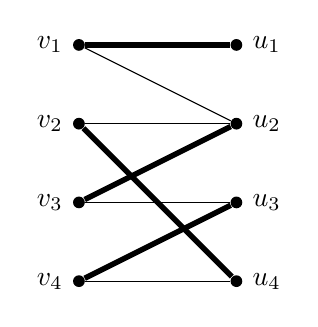
\begin{tikzpicture}
        \node[circle,fill,inner sep=1.5pt,label=left:$v_1$] (v1)  at (0,0) {};
        \node[circle,fill,inner sep=1.5pt,label=left:$v_2$] (v2)  at (0,-1) {};
        \node[circle,fill,inner sep=1.5pt,label=left:$v_3$] (v3)  at (0,-2) {};
        \node[circle,fill,inner sep=1.5pt,label=left:$v_4$] (v4)  at (0,-3) {};

        \node[circle,fill,inner sep=1.5pt,label=right:$u_1$] (u1)  at (2,0) {};
        \node[circle,fill,inner sep=1.5pt,label=right:$u_2$] (u2)  at (2,-1) {};
        \node[circle,fill,inner sep=1.5pt,label=right:$u_3$] (u3)  at (2,-2) {};
        \node[circle,fill,inner sep=1.5pt,label=right:$u_4$] (u4)  at (2,-3) {};

        \path [-] (v1) edge node {}  (u2);
        \path [-] (v2) edge node {}  (u2);
        \path [-] (v3) edge node {}  (u3);
        \path [-] (v4) edge node {}  (u4);

        \path [-, line width=2] (v1) edge node {}  (u1);
        \path [-, line width=2] (v2) edge node {}  (u4);
        \path [-, line width=2] (v3) edge node {}  (u2);
        \path [-, line width=2] (v4) edge node {}  (u3);
    \end{tikzpicture}
    \label{fig:graphs:perfect_match}
    \caption{пример совершенного паросочетания на двудольном графе}
\end{figure}


В случае двудольных графов задача построения паросочетаний и, в частности,
совершенных паросочетаний может быть мотивирована желанием построить взаимнооднозначное соответствие для как можно большего числа вершин из разных долей
(возвращаясь к примеру с работниками и задачами, построение совершенного паросочетания означает наиболее оптимальное распределение задач по работникам).

В этой связи формулируется теорема, гарантирующая существование совершенного паросочетания в двудольном графе при выполнении определённого условия.
Для строгой формулировки этого условия придётся ввести некоторые вспомогательные понятия.

\begin{definition}
    \defemph{Множеством соседей (окрестностью) вершины} $ v $ графа $ G $ будем называть множество $ N(v) = \{ u \mid \{u, v\} \in E(G) \} $
    \newline
    \defemph{Множеством соседей подмножества вершин} $ U \subseteq V(G) $ графа $ G $ будем называть множество $ N(U) = \left( \bigcup_{u \in U} N(u) \right) \setminus U $.
\end{definition}

\begin{theorem}[Холла о свадьбах]
    В двудольном графе с долями $ L $ и $ R $ существует совершенное паросочетание тогда и только тогда,
    когда $ |L| = |R| $ и для любого подмножества $ S \subseteq L $ справедливо $ |N(S)| \geqslant |S| $.
\end{theorem}

\begin{Exercise}[counter=SecExercise, label={exercise:almost_BFS}]
    \noindent
    Пусть $ G $ связный граф, $ v_0 \in V(G) $.
    Пусть $ S_0 = \{ v_0 \} $, $ S_{k+1} = N(S_k) \cup S_k $.
    Задайте множества $ S_k $ явно в терминах расстояний в графе.
    %Найдите минимальное $ k_0 $, при котором $ S_{k_0+1} = S_{k_0} $.
\end{Exercise}

\begin{Answer}
    \noindent
    %Покажем, что $\displaystyle k_0 = \max_{u \in V(G)} \rho(v_0, u) $.

    %Действительно, для этого
    По индукции докажем, что $ S_k = \{ u \in V(G) \mid \rho(v_0, u) \leqslant k \} $.
    \newline
    \textbf{База:}
    $ S_0 = \{ v_0 \} = \{ u \mid \rho(v_0, u) \leqslant 0 \} $ по определению.
    \newline
    \textbf{Шаг:}
    Пусть для $ k $ утверждение истинно.
    Рассмотрим $ k + 1 $.
    Пусть $ \rho(v_0, u) \leqslant k $.
    Тогда $ u \in S_k \subseteq S_{k+1} $.
    %\newline
    Пусть теперь $ \rho(v_0, u) = k + 1 $.
    Кратчайший путь из $ v_0 $ в $ u $ содержит вершину $ u' $, смежную с $ u $ и такую, что $ \rho(v_0, u') = k $.
    Тогда $ u' \in S_k $, из чего следует, что $ u \in N(S_k) \subseteq S_{k+1} $.
    %\newline
    Наконец, пусть $ \rho(v_0, u) > k + 1 $.
    По предположению индукции $ u \notin S_k $.
    Также $ u \notin N(S_k) $, иначе был бы путь из $ v_0 $ в $ u $ длины $ k + 1 $.
    Значит, $ u \notin S_{k+1} $.
    \newline
    По индукции доказано.

    %Из утверждения выше имеем, что $ S_{k+1} \setminus S_{k} = \{ u \mid \rho(v_0, u) = k+1 \} $.
    %Отсюда, если $ S_{k_0+1} = S_{k_0} $, то $ \forall u \in V(G) \;\, \rho(v_0, u) \neq k_0+1 $.
    %Но тогда не имеем путей из $ v_0 $ длины больше $ k_0 $.
    %Это возможно тогда и только тогда, когда $ \displaystyle k_0 \geqslant \max_{u \in V(G)} \rho(v_0, u) $.
    %Отсюда получаем ответ.
\end{Answer}

\begin{Exercise}[counter=SecExercise]
    \noindent
    Используя задачу \ref{exercise:almost_BFS}, постройте алгоритм поиска кратчайших путей из заданной вершины во все остальные в простом неориентированном графе.
\end{Exercise}



\newpage



\section{Ориентированные графы}
\label{sec:oriented_graphs}

\defemph{Ориентированные графы}~--- естественное обобщение неориентированных.
Они получаеются простой заменой неупорядоченной пары на упорядоченную в определении ребра:
\begin{definition}
    \defemph{Ориентированный граф (возможно, с петлями)}~--- это упорядоченная пара $ (V, E) $ множества \defemph{вершин} $ V $
    и \defemph{рёбер} $ E \subseteq V^2 $.
    В дальнейшем будет подразумеваться, что в ориентированном графе петель нет, то есть $ E \cap \{(v, v) \mid v \in V \} = \varnothing $.
\end{definition}

Определения, введённые нами для неориентированных графов, с поправками переносятся на ориентированные.

\begin{definition}
    \defemph{Исходящей степенью} $ d_+(v) $ вершины $ v $ называется число рёбер, началом которых является $ v $,
    то есть $ d_+(v) = |\{ (v, u) \mid u \in V \}| $.
    Симметрично вводится понятие \defemph{входящей степени} $ d_-(v) $ вершины $ v $: $ d_-(v) = |\{ (u, v) \mid u \in V \}| $.
\end{definition}

Для ориентированного графа есть утверждение, аналогичное теореме \ref{theorem:graphs:sum_of_degs} о рукопожатиях:

\begin{statement}
    $ \displaystyle \sum_{v \in V} d_+(v) = \sum_{v \in V} d_-(v) = |E| $
\end{statement}

Определим отдельно несколько частных случаев простого неориентированного графа.
\begin{definition}
    \begin{enumerate}[label=\arabic*)]
        \item[]
        \item
            \defemph{Ориентированный граф-путь} $ P_n $, $ n \geqslant 0 $~--- граф вида
            \[
                V(P_n) = \{ v_1, \ldots, v_n \}, \qquad
                E(P_n) = \left\{ (v_0, v_1), (v_1, v_2), \ldots, (v_{n-1}, v_n) \right\}
            \]
            Вершины $ v_1 $ и $ v_n $ называются \defemph{концами пути}, а $ n = |E| $~--- \defemph{длиной}.
            \textit{Ещё раз акцентируем внимание на том, что $ n \geqslant 0 $, а вершины нумеруются с нуля.}
        \item
            \defemph{Ориентированный граф-цикл} $ C_n $, $ n \geqslant 2 $~--- граф вида
            \[
                V(G) = \{ v_1, \ldots, v_n \}, \qquad
                E(G) = \left\{ (v_1, v_2), (v_2, v_3), \ldots, (v_{n-1}, v_n), (v_n, v_1) \right\}
            \]
            \textit{Ещё раз акцентируем внимание на том, что \uline{в отличие от неориентированного графа-цикла}, $ n \geqslant 2 $.}
    \end{enumerate}
\end{definition}

Без изменений вводится понятие подграфа ориентированного графа, а также индуцированного графа.

\begin{definition}
    Ориентированный граф, в котором нет подграфов-циклов, является \defemph{ациклическим}.
\end{definition}

\begin{definition}
    Вершина $ u $ в ориентированном графе $ G $ является \defemph{достижимой} из вершины $ v $ $ \defarr $ существует подграф-путь графа $ G $,
    концами которого являются вершины $ u $ и $ v $.
    Это обозначается как $ u \leadsto v $.
\end{definition}

Из свойств, описанных в замечании \ref{remark:graphs:connectivity_relation},
для ориентированного сохраняются только \emph{рефлексивность} и \emph{транзитивность};
симметричности в общем случае нет.
Однако понятие достижимости для ориентированного графа можно симметризовать:

\begin{definition}
    Вершины $ u $ и $ v $ являются \defemph{двусторонне достижимыми} $ \defarr $ $ (u \leadsto v) \wedge (v \leadsto u) $.
    Это обозначается как $ u \connected v $.
\end{definition}

Для отношения двусторонней достижимости можно ввести понятие \defemph{компонент сильной связности}, аналогичное \ref{definition:graphs:connectivity_component}:

\begin{definition}
    \label{definition:oriented_graphs:strong_connectivity_component}
    \defemph{Компонентой сильной связности} ориентированного графа $ G(V, E) $ будем называть подграф $ G $,
    индуцированный на некотором \underline{непустом} множестве $ U \subseteq V $,
    удовлетворяющем свойству $ \forall u, v \in U \; (u \connected v) $ и являющемся максимальным относительно него.
\end{definition}

\begin{definition}
    \defemph{Маршрутом} длины $ n \geqslant 0 $ в ориентированном графе $ G $ называется последовательность вершин $ v_0, v_1, \ldots, v_n $ такая,
    что $ \forall i \in \{ 0, \ldots, n-1 \} \;\, \left( (v_i, v_{i+1}) \in E(G) \right) $.
    \newline
    Число $ n $ называется \defemph{длиной маршрута}.
    \newline
    \textit{Отметим отдельно, что одна вершина тоже является маршрутом длины $ 0 $.}
    \\[0.25\baselineskip]
    Вершины $ v_0 $ и $ v_n $ называются \defemph{концами} маршрута;
    говорится, что маршрут \defemph{соединяет} $ v_0 $ и $ v_n $.
    В случае $ v_0 = v_n $ маршрут является \defemph{замкнутым}.
    \newline
    Говорят, что ребро $ (x, y) \in E(G) $ \defemph{лежит} на маршруте, если $ \exists i: \; (x, y) = (v_i, v_{i+1}) $.
\end{definition}

С учётом введённых определений утверждение \ref{statement:graphs:path_walk_equivalency} справедливо и для ориентированного графа.
Также можно сформулировать замечание, аналогичное \ref{remark:graphs:cc_partition}.

Введём теперь новое определение, которое можно обобщить и на случай неориентированного графа:
\begin{definition}
    Два графа $ G(V, E) $ и $ G'(V', E') $ называются \defemph{изоморфными} $ \defarr $ существует биекция $ f: V \to V' $ такая,
    что $ \forall (u, v) \in E \; \left[ (f(u), f(v)) \in E' \right] $.
\end{definition}
